\documentclass[../main.tex]{subfiles}

\begin{document}

The selection of certain laser wavelengths can be achived with the introdcution of artificial losses for the undesired remaining wavelengths.

\subsubsection{Birefringent tuner}
    \paragraph{Methodology}
        One possible realisation for these losses is using a birefringent quartz crystal ($n_Q \approx\num{1.55}$ for the main laser line of $\lambda = \SI{633}{nm}$). The setup used in the experiment is shown in figure \ref{fig:5-Aufbau}.

        \begin{figure}[H]
            \centering 
            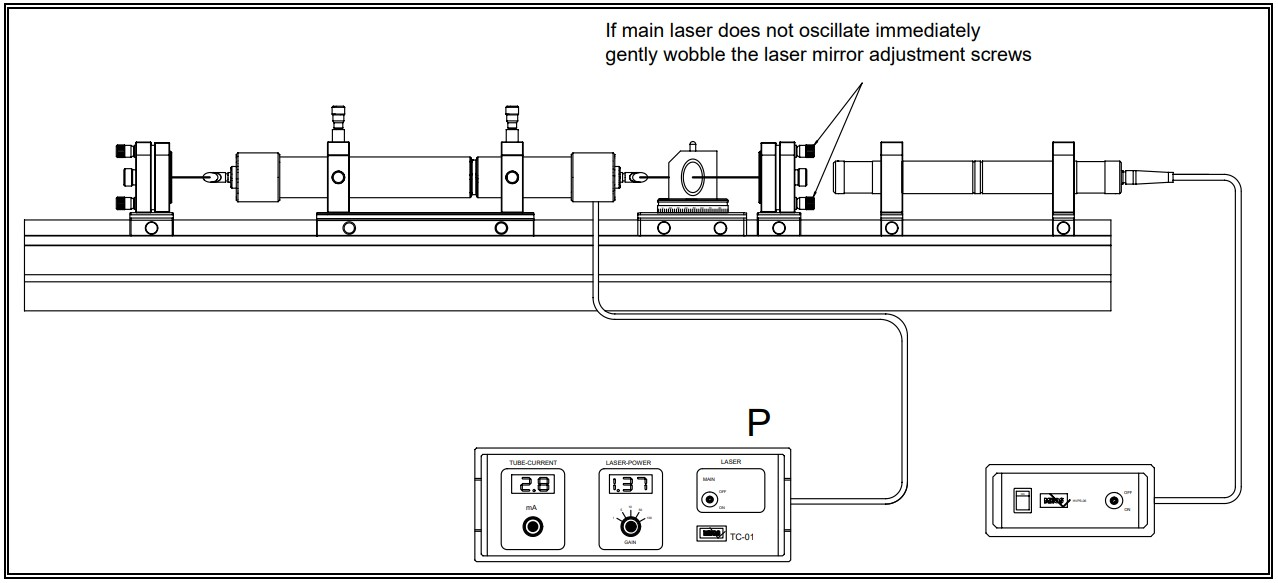
\includegraphics[width = 11cm]{Bilddateien/5-Aufbau.jpg}
            \caption{ Experimental setup for the selection of certain laser wavelengths. The components displayed are from left to right: left laser mirror holder (A), main laser tube (B), birefringent tuner (C), right laser mirror holder (D), pilot laser (E). For the measurment of the laser spectrum a spectrometer can be placed left to the left laser mirror holder (A).}
            \label{fig:5-Aufbau}
        \end{figure}

    \paragraph{Data analysis}

    The observed wavelengths and corresponding probable transitions of Neon gas particle are listed in table \ref{tab:6-Birefringent-peaks}.

    \begin{table}[H]
        \centering 
        \begin{tabular}{c | c c}
            \textbf{Wavelength} & \textbf{Times observed} & \textbf{Correlated transtion}\\\hline\hline
            \SI{633.0(10)}{\nm} & 6 & $3S^2\to 2p^4$\\
            \SI{640.0(10)}{\nm} & 2 & $3S^2\to 2p^2$
        \end{tabular}
        \caption{Observed spectral peaks in the lasing spectrum filtered with a birefringent crystal. The wavelengths listed are mean values of all observed occurences. For the uncertainty the distance between neighbouring Wavelength values in the discretised spectrum.}
        \label{tab:6-Birefringent-peaks}
    \end{table}

\subsubsection{Littrow prism tuner}
    \paragraph{Methodology}
    \paragraph{Data analysis}

\subsubsection{spectra of the laser light}
    \paragraph{Methodology}
    Lastly, a more indirect approach to wavelength 'selection' is taken, which does not focus on actually seperating a single wavelength, but instead on taking the laser spectrum under the microscope. For this, the birefringent crystal (C) is removed from the setup shown in figure \ref{fig:5-Aufbau}. The spectrometer is then placed right next to the main laser tube (B) and a spectrum is taking for two cases: once for when lasing is occuring, and once for when the lasing process is being blocked. The difference between both spectra gives insight into the induced emissions in the Neon gas essential to the function of a laser.

    \paragraph{Data analysis}

    Firstly, the figure shows the laser/ pure fluorescence spectrum for both the case of lasing and no lasing. It is important to note that the spectrum corresponds to that of the light scattered due to \textit{incoherent} emissions in the Neon-Helium gas mixture.

    \begin{figure}[H]
        \centering 
        \includegraphics[width = 11cm]{Bilddateien/5-NeonSpektren.jpg}
        \caption{Incoherent scattering spectrum for HeNe-gas. Three main peaks, marked with a red line each, were observed in total. In order of ascending intensity, these peaks occured at \SI{668}{\nm}, \SI{588}{\nm} and \SI{638}{\nm}.}
        \label{fig:5-NeonSpektren}
    \end{figure}

    Interestingely, the three larget peaks in spectrum \ref{fig:5-NeonSpektren} do not correspond to any possible transitions in the 


\end{document}